\documentclass[a4paper, 11pt]{amsart}

%\usepackage[T1]{fontenc}
\usepackage{geometry}
\geometry{verbose,letterpaper,tmargin= 1in,bmargin=1in,lmargin=1in,rmargin=1in}
\usepackage{wrapfig}
\usepackage{multicol}
\usepackage{enumerate}   
\usepackage{enumitem}
\usepackage{graphicx}
\usepackage{soul}
\usepackage{xcolor}
\usepackage{amssymb}
\def\e{{\epsilon}}
\def\ra{{\rightarrow}}
\def\tr{{\rm tr}}
\newtheorem{theorem}{Theorem}[section]
\newtheorem{lemma}[theorem]{Lemma}
\newtheorem{proposition}[theorem]{Proposition}
\newtheorem{corollary}[theorem]{Corollary}
{ \theoremstyle{definition}
\newtheorem{definition}[theorem]{Definition}}
%{ \theoremstyle{definition} \newtheorem{conjecture}[theorem]{Conjecture}}
{ \theoremstyle{remark}
\newtheorem{remark}[theorem]{Remark}}
\usepackage{placeins}
%\usepackage{bbm}
\setcounter{tocdepth}{1}
\usepackage{cite}
\usepackage{caption}
\usepackage{enumerate}
\usepackage{afterpage}
\usepackage{enumitem}
%\usepackage[dvipdfmx]{graphicx} 
\usepackage{bmpsize}
\usepackage{hyperref}
\usepackage{enumitem}   
\usepackage[framemethod=tikz]{mdframed}
\pagenumbering{gobble}

\newcounter{theo}[section]\setcounter{theo}{0}
\renewcommand{\thetheo}{\arabic{section}.\arabic{theo}}
\newenvironment{theo}[2][]{%
\refstepcounter{theo}%
\ifstrempty{#1}%
{\mdfsetup{%
frametitle={%
\tikz[baseline=(current bounding box.east),outer sep=0pt]
\node[anchor=east,rectangle,fill=blue!20]
{\strut Problem~\thetheo};}}
}%
{\mdfsetup{%
frametitle={%
\tikz[baseline=(current bounding box.east),outer sep=0pt]
\node[anchor=east,rectangle,fill=blue!20]
{\strut Problem~\thetheo ~#1};}}%
}%
\mdfsetup{innertopmargin=0pt,linecolor=blue!20,%
linewidth=2pt,topline=true,%
frametitleaboveskip=\dimexpr-\ht\strutbox\relax
}
\begin{mdframed}[]\relax%
\label{#2}}{\end{mdframed}}


\usepackage{tikz}

\usetikzlibrary{matrix,graphs,arrows,positioning,calc,decorations.markings,shapes.symbols}

% \usepackage{tikz-cd}

\definecolor{dullmagenta}{rgb}{0.4,0,0.4} % #660066

\definecolor{darkblue}{rgb}{0,0,0.4}

\newenvironment{lem}[2][]{%
\ifstrempty{#1}%
{\mdfsetup{%
frametitle={%
\tikz[baseline=(current bounding box.east),outer sep=0pt]
\node[anchor=east,rectangle,fill=red!20]
{\strut Approach~};}}
}%
{\mdfsetup{%
frametitle={%
\tikz[baseline=(current bounding box.east),outer sep=0pt]
\node[anchor=east,rectangle,fill=red!20]
{\strut Approach ~#1};}}%
}%
\mdfsetup{innertopmargin=0pt,linecolor=red!20,%
linewidth=2pt,topline=true,%
frametitleaboveskip=\dimexpr-\ht\strutbox\relax
}
\begin{mdframed}[]\relax%
\label{#2}}{\end{mdframed}}


%\usepackage[dvips]{color}

% Color Information from - http://www-h.eng.cam.ac.uk/help/tpl/textprocessing/latex_advanced/node13.html



%\textheight9.5in
%\textwidth6.75in
%\newcommand\bb[1]{\mbox{\em #1}}
\def\baselinestretch{1.05}
%\pagestyle{empty}
%\pagenumbering{gobble}
\newcommand{\hsp}{\hspace*{\parindent}}
\definecolor{gray}{rgb}{0.4,0.4,0.4}
%\definecolor{gray}{rgb}{1.0,1.0,1.0}
\setlength{\footskip}{30pt}


\begin{document}









\begin{center}
\Large Title: Asymptotics of Bernoulli Gibbsian line ensembles\\
\Large Project Leader: Evgeni Dimitrov
\end{center}

\vspace{15mm}

{\raggedleft \bf Gibbs measures.} Many problems in probability theory and mathematical physics deal with random objects, whose distribution has a {\em Gibbs property}. The term ``Gibbs" means different things in different contexts, and to illustrate what we mean by it we consider a simple model of lozenge tilings of the hexagon. Consider three integers $A, B, C\geq 1$ and the $A \times B \times C$ hexagon drawn on the triangular lattice, see the left part of Figure \ref{S1_1}. By gluing two triangles along a common side, we obtain three types of tiles (also called {\em lozenges}), that are depicted in red, blue and green on the left part of Figure \ref{S1_1}. There are finitely many possible ways to tile any given hexagon and we can put the uniform measure on all such tilings. The resulting random tiling model satisfies the following Gibbs property: if we fix a tileable region $K$ in the hexagon, and fix the tiling outside of it then the conditional distribution of the tilings of $K$ is just the uniform measure on all possible tilings of $K$. See the right part of Figure \ref{S1_1}.
\begin{figure}[h]
\begin{center}
  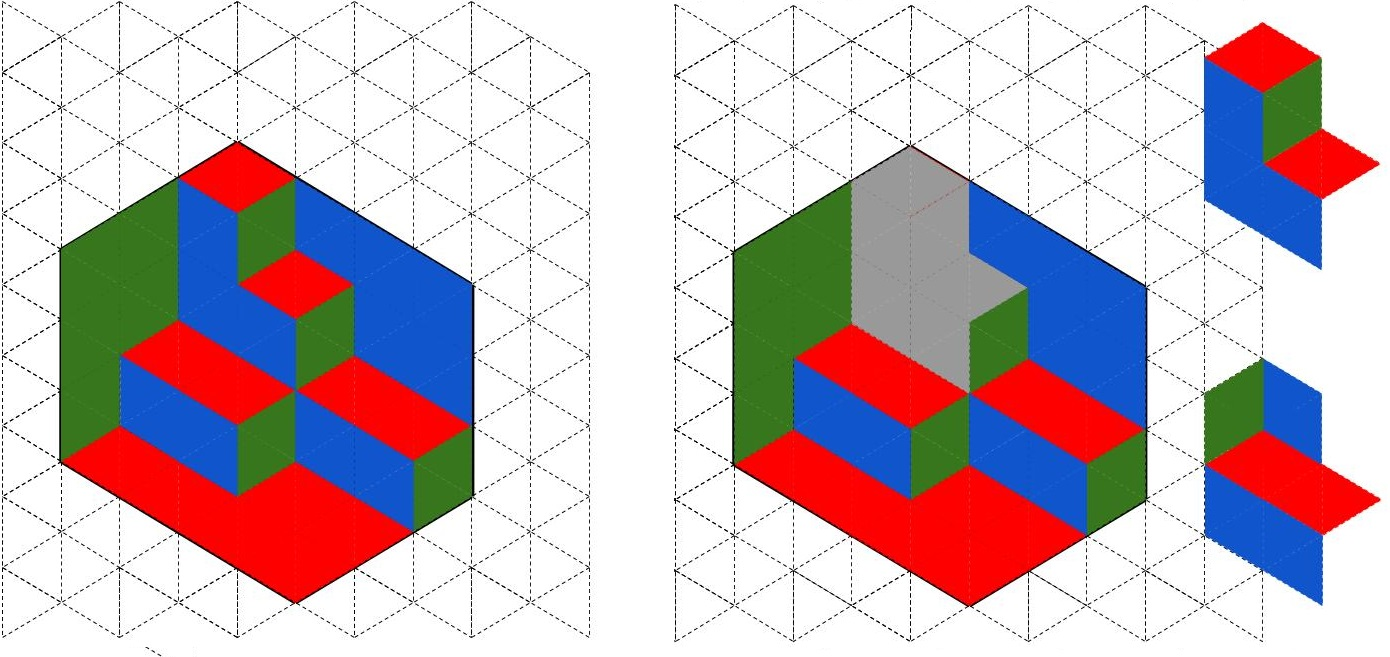
\includegraphics[scale = 0.40]{S_2.jpg}
  \vspace{-2mm}
  \caption{ The left part depicts a $3 \times 3 \times 4$ hexagon with a particular tiling. On the right side, a tilable region $K$ is depicted in grey. There are two possible ways to tile $K$, given the tiling outside of it (they are drawn on the very right of the picture). The Gibbs property says that each of these two tilings is equally likely; i.e. the probability of seing either one in $K$, conditional on the given tiling outside of $K$, is equal to $1/2$. }
  \label{S1_1}
  \end{center}
\end{figure}

{\raggedleft \bf Gibbsian line ensembles.} There is a natural way to rephrase the above hexagon tiling model and its Gibbs property in terms of random walks, see Figure \ref{S1_2}. Namely, we can put a line connecting the mid-points of the left and right sides of each of the green and blue lozenges. In this way we obtain $A$ random curves connecting the left and right side of the hexagon. A natural way to interpret these curves is as trajectories of three Bernoulli random walks, whose starting and ending points are the yellow dots on the two sides of the hexagon, and which have been conditioned to never intersect. Let us perform a simple affine transformation of the picture and introduce cooridnate axes, see Figure \ref{Fig1}.  
\begin{figure}[h]
\begin{center}
  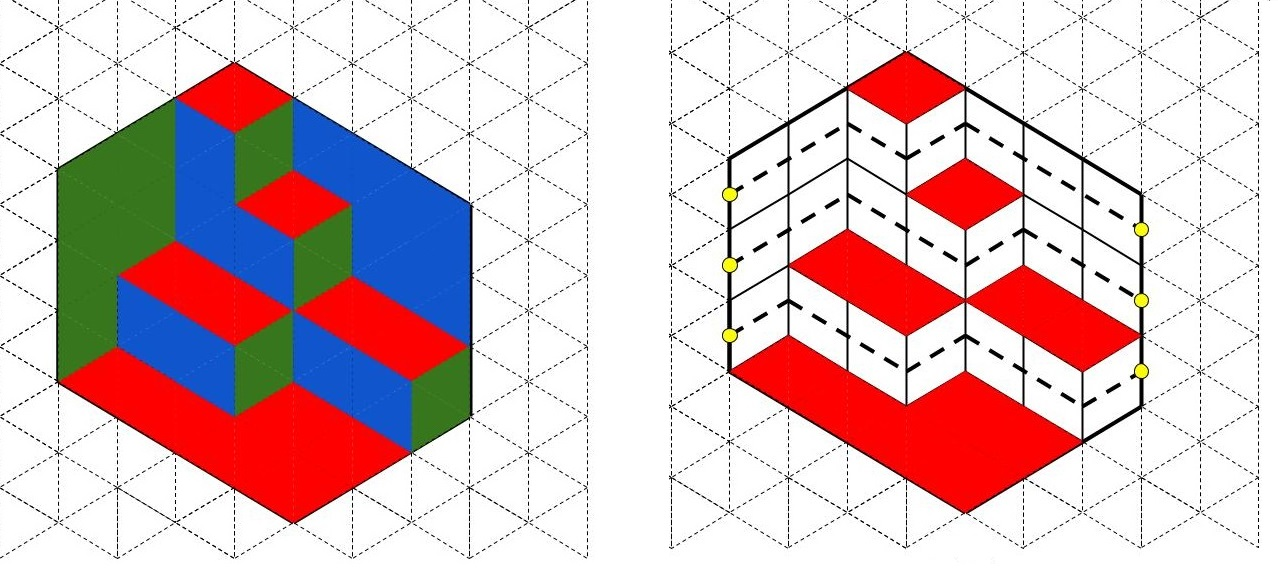
\includegraphics[scale = 0.40]{S_1.jpg}
  \vspace{-2mm}
  \caption{ The left part depicts a $3 \times 3 \times 4$ hexagon with a particular tiling. On the right side, we have the reinterpretation of the tiling as a collection of trajectories of three Bernoulli random walks, conditioned on non-intersecting. }
  \label{S1_2}
  \end{center}
\end{figure}

\begin{figure}[h]
\centering
\begin{tikzpicture}[>=stealth,
brxy/.style={fill=yellow!30!white, draw=yellow!30!black},
bryz/.style={fill=blue!18!white, draw=blue!30!black},
brxz/.style={fill=red!60!white, draw=red!30!black},
pth/.style={very thick, draw=black},
intpt/.style={circle, draw=white!100, fill=purple!70!black, very thick, inner sep=1pt, minimum size=2.5mm},
scale=0.7
]
\def\brxy(#1:#2:#3){
\filldraw[brxy]
(${(#1)+0}*(1,0) + {(#2)+0}*({sqrt(2)*cos(deg(pi/4))},{sqrt(2)*sin(deg(pi/4))}) + {(#3)-0.5}*(0,1)$) --
(${(#1)+1}*(1,0) + {(#2)+0}*({sqrt(2)*cos(deg(pi/4))},{sqrt(2)*sin(deg(pi/4))}) + {(#3)-0.5}*(0,1)$) --
(${(#1)+1}*(1,0) + {(#2)+1}*({sqrt(2)*cos(deg(pi/4))},{sqrt(2)*sin(deg(pi/4))}) + {(#3)-0.5}*(0,1)$) --
(${(#1)+0}*(1,0) + {(#2)+1}*({sqrt(2)*cos(deg(pi/4))},{sqrt(2)*sin(deg(pi/4))}) + {(#3)-0.5}*(0,1)$) -- cycle;
}
\def\bryz(#1:#2:#3){
\filldraw[bryz]
(${(#1)+0}*(1,0) + {(#2)+0}*({sqrt(2)*cos(deg(pi/4))},{sqrt(2)*sin(deg(pi/4))}) + {(#3)-0.5}*(0,1)$) --
(${(#1)+0}*(1,0) + {(#2)+1}*({sqrt(2)*cos(deg(pi/4))},{sqrt(2)*sin(deg(pi/4))}) + {(#3)-0.5}*(0,1)$) --
(${(#1)+0}*(1,0) + {(#2)+1}*({sqrt(2)*cos(deg(pi/4))},{sqrt(2)*sin(deg(pi/4))}) + {(#3)+0.5}*(0,1)$) --
(${(#1)+0}*(1,0) + {(#2)+0}*({sqrt(2)*cos(deg(pi/4))},{sqrt(2)*sin(deg(pi/4))}) + {(#3)+0.5}*(0,1)$) -- cycle;
\draw[pth]
(${(#1)+0}*(1,0) + {(#2)+0}*({sqrt(2)*cos(deg(pi/4))},{sqrt(2)*sin(deg(pi/4))}) + {(#3)}*(0,1)$) --
(${(#1)+0}*(1,0) + {(#2)+1}*({sqrt(2)*cos(deg(pi/4))},{sqrt(2)*sin(deg(pi/4))}) + {(#3)}*(0,1)$);
}
\def\brxz(#1:#2:#3){
\filldraw[brxz]
(${(#1)+0}*(1,0) + {(#2)+0}*({sqrt(2)*cos(deg(pi/4))},{sqrt(2)*sin(deg(pi/4))}) + {(#3)-0.5}*(0,1)$) --
(${(#1)+1}*(1,0) + {(#2)+0}*({sqrt(2)*cos(deg(pi/4))},{sqrt(2)*sin(deg(pi/4))}) + {(#3)-0.5}*(0,1)$) --
(${(#1)+1}*(1,0) + {(#2)+0}*({sqrt(2)*cos(deg(pi/4))},{sqrt(2)*sin(deg(pi/4))}) + {(#3)+0.5}*(0,1)$) --
(${(#1)+0}*(1,0) + {(#2)+0}*({sqrt(2)*cos(deg(pi/4))},{sqrt(2)*sin(deg(pi/4))}) + {(#3)+0.5}*(0,1)$) -- cycle;
\draw[pth]
(${(#1)+0}*(1,0) + {(#2)+0}*({sqrt(2)*cos(deg(pi/4))},{sqrt(2)*sin(deg(pi/4))}) + {(#3)}*(0,1)$) --
(${(#1)+1}*(1,0) + {(#2)+0}*({sqrt(2)*cos(deg(pi/4))},{sqrt(2)*sin(deg(pi/4))}) + {(#3)}*(0,1)$);
}
\brxy(0:1:3);\brxy(0:2:3);\brxy(1:2:3);\brxz(2:3:2);\brxz(3:3:2);
\bryz(0:0:2);\brxz(0:1:2);\bryz(1:1:2);\brxy(1:1:2);\brxz(1:2:2);\brxy(2:2:2);\bryz(2:2:2);
\bryz(0:0:1);\brxz(0:1:1);\brxz(1:1:1);\bryz(2:1:1);\brxz(2:2:1);\bryz(3:2:1);\brxz(3:3:1);
\brxy(0:0:1);\brxy(1:0:1);\brxy(2:0:1);\brxy(2:1:1);\brxy(3:0:1);\brxy(3:1:1);\brxy(3:2:1);
\brxz(0:0:0);\brxz(1:0:0);\brxz(2:0:0);\brxz(3:0:0);\bryz(4:0:0);\bryz(4:1:0);\bryz(4:2:0);
% Create the axes
\draw[->] (-0.5,0) -- (8,0) node[right] {$t$};
\draw[->] (0,-0.5) -- (0,6.5) node[above] {$x$};
% Create the time slice
\draw[-,line width=0pt] (3,6) -- (3,-1) node[below] {$t=3$};
\node[intpt] at (3,0) {}; \node[intpt] at (3,2) {}; \node[intpt] at (3,4) {};
\end{tikzpicture}
\caption{Lozenge tiling of the hexagon and corresponding up-right path configuration. The dots represent the location of the random walks at time $t = 3$.} \label{Fig1}
\end{figure} 
Let us number the random paths from top to bottom by $L_1, L_2, \dots, L_A$, and denote the position of the $k$-th random walk at time $t$ by $L_k(t)$. Then the Gibbs property for the tiling model, can be seen to be equivalent to the following statement. Suppose that we sample $\{L_m\}_{m = 1}^A$ and fix two times $0 \leq s < t \leq B+C$ and an index $k \in \{1, \dots, A\}$. We can erase the part of the path $L_k$ between the points $(s, L_k(s))$ and $(t, L_k(t))$ and sample independently a new up right path between these two points uniformly from the set of all such paths that do not intersect the lines $L_{k-1}$ and $L_{k + 1}$ with the convention that $L_{0} = \infty$ and $L_{A+1} = -\infty$. In this way we obtain a new random collection of paths $\{L'_m\}_{m = 1}^A$ whose law is readily seen to be the same as that of $\{L_m\}_{m = 1}^A$. We refer to the latter as the {\em Bernoulli Gibbs property} and refer to probability distributions that satisfy it as {\em Bernoulli Gibbsian line ensembles}. 

At this point one can abandon the lozenge tiling model altogether and consider in general laws on (possibly infinitely) many continuous curves that satisfy the Bernoulli Gibbs property. What we will be interested in understanding the asymptotic behavior of these line ensembles. In the context of the above hexagon tiling model, asymptotic refers to setting $A = \lfloor a \cdot L \rfloor$, $B = \lfloor b \cdot L \rfloor $ and $C = \lfloor c \cdot L \rfloor $ where $a,b,c > 0$ and sending $L \rightarrow \infty$. In more general settings we will consider other types of asymptotics. As will be explained in the initial stages of the project, the limiting behavior of  {Bernoulli Gibbsian line ensembles} is governed by what is called the {\em Airy line ensemble}, which is a certain random collection of infinitely many Brownian motions, conditioned on not intersecting. The purpose of this project is then to give sufficient conditions, under which, given a sequence of Bernoulli Gibbsian line ensembles they converge to the Airy line ensemble.\\

{\raggedleft \bf Project outline.} The goals of the project will be to:
\begin{enumerate}
\item Understand some of the combinatorial structures behind hexagon tiling models and Bernoulli random walks. Here we will learn bits of symmetric function theory.
\item Understand some classical notions of convergence of random variables, random vectors and random continuous curves. Here we will learn some advanced probability theory and topology.
\item Establish monotone coupling results for Bernoulli Gibbsian line ensembles.
\item Use some existing strong coupling results for Bernoulli random walk brdiges and Brownian bridges to obtain various estimates for Bernoulli Gibbsian line ensembles.
\item Show that finite-dimensional convergence of the top curve of Bernoulli Gibbsian line ensembles implies convergence of the full line ensembles.
\end{enumerate}


The above project is in a very active area of probability theory, called {\em integrable probability}. One of the goals of the project is to introduce the participants to this area. The problem we are considering was studied very recently in https://arxiv.org/abs/1907.10160, where the authors assumed much stronger conditions than the ones we are considering. One of the reasons, we will be able to improve on their results is due to an upcoming paper by the project leader and Konstantin Matetski. Given, that the project is quite ambitious, it is strongly preferred that candidates have taken at least an undergraduate probability theory class -- MATH GU4155 or some equivalent. Students are expected to know at least some of the basic properties of Brownian motion, weak convergence of random variables and Markov chains. I would be happy to suggest some reading to interested candidates.


\end{document}